
\RequirePackage{plautopatch}  % pLaTeX または upLaTeX のとき
%\documentclass[uplatex,dvipdfmx,titlepage,a4j]{jsarticle}% upLaTeX のとき
\documentclass[dvipdfmx,titlepage,a4j]{jsarticle}  % pLaTeX のとき
\usepackage{listings,jvlisting}
\usepackage{amsmath,amssymb}
\usepackage{graphicx}
\usepackage[yen]{okuverb}
\usepackage{r04ec-exp}
\usepackage{here}
\usepackage{ascmac}
\usepackage{fancybox}
\usepackage{fancyvrb}
\usepackage{fancyhdr}
\usepackage{lastpage}
\usepackage{cases}
\usepackage[hang,small,bf]{caption}
\usepackage[subrefformat=parens]{subcaption}

\fancypagestyle{foot}
{
\fancyhead[C]{電気自動車充電器・メガソーラ発電設備等の高周波騒音の軽減}
\fancyhead[L]{}
\fancyhead[R]{}
\fancyfoot[C]{\thepage / \pageref{LastPage}}
\renewcommand\headrulewidth{0.4pt}
}

%ここからソースコードの表示に関する設定
\lstset{
  language={C++},
  basicstyle={\ttfamily},
  identifierstyle={\small},
  commentstyle={\smallitshape},
  keywordstyle={\small\bfseries},
  ndkeywordstyle={\small},
  stringstyle={\small\ttfamily},
  frame={tb},
  tabsize={2},
  breaklines=true,
  columns=[l]{fullflexible},
  numbers=left,
  xrightmargin=0zw,
  xleftmargin=3zw,
  numberstyle={\scriptsize},
  stepnumber=1,
  numbersep=1zw,
  lineskip=-0.5ex
}

\renewcommand{\lstlistingname}{リスト}
%ここまでソースコードの表示に関する設定

\title{フーリエ解析}
% 学年・番号
\grade{4年42番}%
% 氏名
\author{鷲尾 優作}
% 班(後期は班に分かれて実験をする.そのときは,ここに班番号を記入する.)
\team{}
% 提出日
\date{2023年1月31日}
% 実験日
\expdate{2023年1月5日,1月19日} 
% 共同実験者
% グループに分かれて実験をするテーマでは,グループメンバーの番号名前を書く.
\coauthor{
}
%
%記載例:
%\coauthor{%
%  2番 & 新潟 花子\\
%  11番 & 三条 次郎}
%%

\begin{document}
\pagestyle{foot}

\maketitle

\section{研究テーマ}
電気自動車充電器・メガソーラ発電設備等の高周波騒音の軽減

\section{背景・目的}
再生可能エネルギーの普及に伴い,日本各地で大電力を扱う設備が日常に溶け込む形で普及しつつあるなか,近年問題となっているのが励磁音である.
励磁音を発生させる代表的な装置であるパワコンユニットを備えた設備を図\ref{fig:reijion}に示す.

\begin{figure}[H]
  \centering
  \begin{minipage}{8cm}
    \centering
    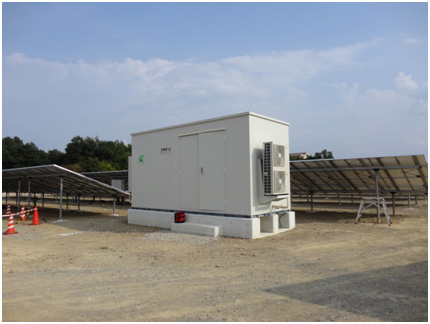
\includegraphics[keepaspectratio, scale=0.4]{../picture/z1.jpg}
    \subcaption{メガソーラー発電所のパワコンユニット}
  \end{minipage}
  \begin{minipage}{8cm}
    \centering
    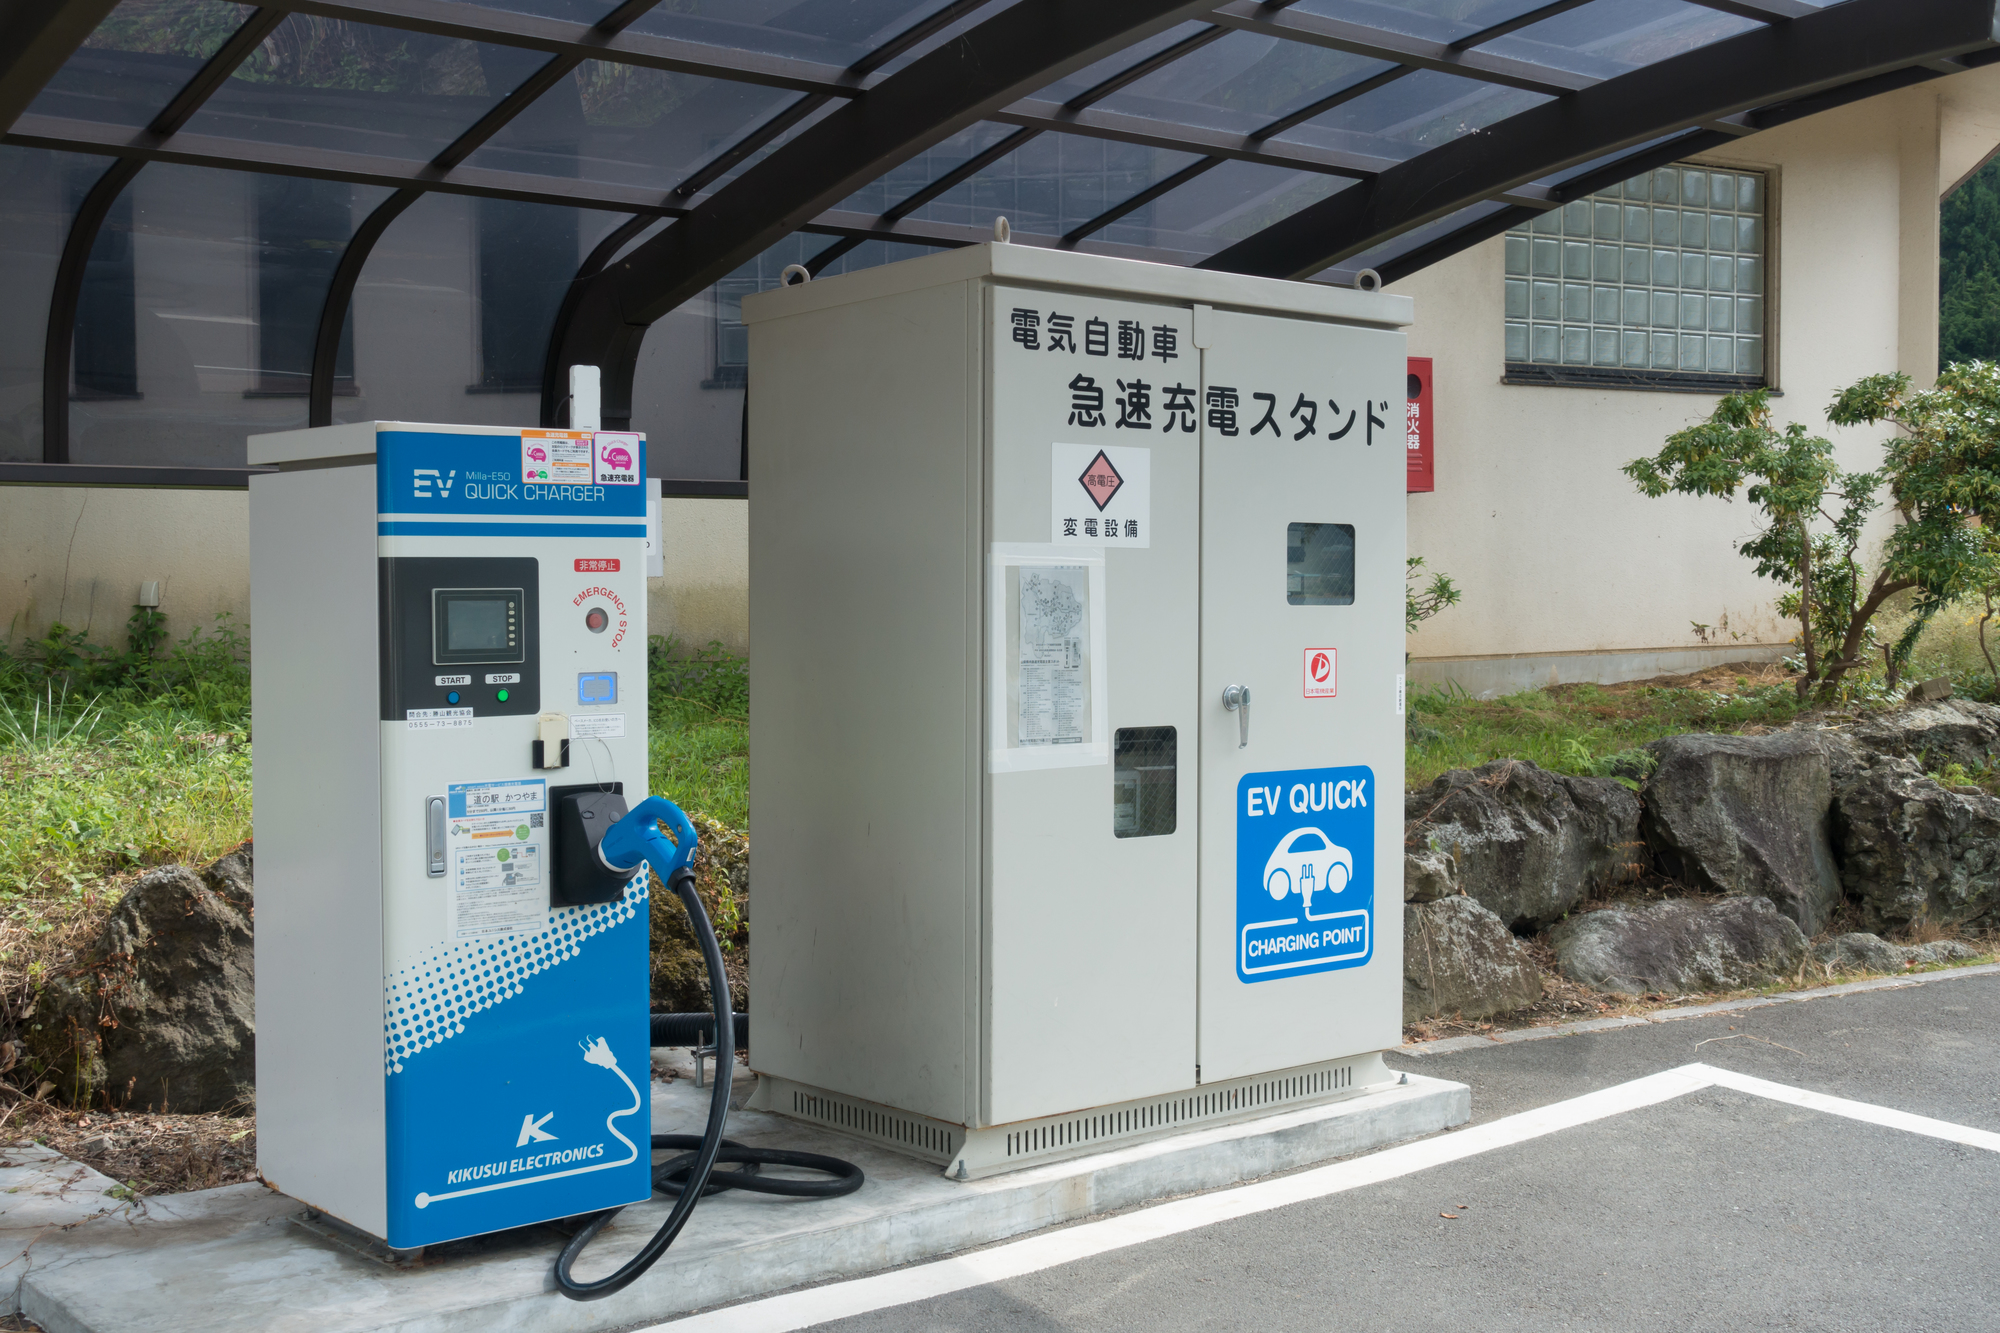
\includegraphics[keepaspectratio, scale=0.4]{../picture/pixta_38502286_M.jpg}
    \subcaption{電気自動車急速充電器}
  \end{minipage}
  \caption{励磁音の発生源}
  \label{fig:reijion}
\end{figure}

パワコンユニットは、送電ネットワークと蓄電に向いた直流の変換を担う装置である.
山間部のメガソーラー発電所のほか,都市部に設置された電気自動車急速充電器に使用され,動作中はキーンという高周波の音を発生させ,近隣住民とのトラブルの誘因に加え,生態系への影響も懸念されている.同様の家庭用設備では睡眠障害を引き起こすなど実生活に被害をもたらす問題であるといえる.

本実験では,生態系や人間の生活に対する発電設備の共存能力を向上させるため、励磁音の特性を解析し,騒音成分を軽減する方法を検討する.

\section{解析手法の検討}
\subsection{励磁音の発生源特定}

有効に励磁音を軽減するためには,励磁音の発生源を詳細に特定することが必要となる.
しかしながら本実験では,パワコンユニットを分解することは不可能であるため,パワコンユニットの内部にあるコイルや電極の振動を直接測定することは困難である.

一般的な考え方として,励磁音がパワコンユニットの内部にある複数のコイルや電極の振動によって発生していると仮定する.
この場合,パワコンユニット外部に流れる励磁音は,各発生源の振動によって発生する励磁音の和であると推定される.
今回はこの予測に基づき,パワコンユニット外部に流れる励磁音を測定し,フーリエ変換により励磁音の周波数特性を解析,発生源を特定することを目指す.

\subsection{離散フーリエ変換(DFT)}
コンピュータ上でフーリエ変換による周波数解析を実現する方法として,離散フーリエ変換(DFT)がある.
DFTは,本来連続関数に適用するフーリエ変換を,マイクロフォン等から取得した離散的な時系列データの解析に用いるためのアルゴリズムである.
実装が比較的容易であること,入力するデータの特性を考慮し,本実験ではDFTを用いて励磁音の周波数特性を解析する.

\paragraph{離散フーリエ変換の理論\\}
離散フーリエ変換の理論について述べる.
前提として連続関数に適用するフーリエ変換は,有限区間[$-T/2$, $T/2$]において式\ref{eq:fourier}で表される.
\begin{equation}
F(\omega) = \int_{-T/2}^{T/2} f(t) e^{-i\omega t} dt
\label{eq:fourier}
\end{equation}

しかしながら,離散的な時系列データに対して式\ref{eq:fourier}を適用すると積分計算が実施できず,0が出力されてしまう.
離散フーリエ変換は,この問題を解決するため入力信号のサンプリング周期に合わせ,複素フーリエ級数を用いて式\ref{eq:fourier}を近似するものである.
式\ref{eq:fourier}を複素フーリエ級数で近似すると,各周波数$\omega$におけるフーリエ成分$F(\omega)$は式\ref{eq:dft}で表される.
\begin{equation}
  F(\omega) = \sum_{n=0}^{N-1} f(n) e^{-i\omega n}
\label{eq:dft}
\end{equation}

\paragraph{アルゴリズムの実装\\}
上記アルゴリズムを実装するために,RustによるDFTの関数を作成した.Rustは,C/C++と同様に高速な実行速度を実現することができることに加え,メモリの安全性を保証することができる言語である.
将来的なFFTへの改造を考慮し,Rustを用いて実装した.
入力する時系列データは64bitの浮動小数点数を想定している.

リスト\ref{fourier.rs}に作成したRustによるDFTの関数実装を示す.

\lstinputlisting[caption=fourier.rs,label=fourier.rs,firstline=1,lastline=19,firstnumber=1,]
{../src/fourier.rs}

関数の入力と出力は,それぞれ入力信号$f(n)$と各周波数$\omega$におけるフーリエ成分$F(\omega)$とする.
関数の入力として,可変長の入力信号$f(n)$の時系列ベクタframesと入力信号のサンプリング周期sampling\_freqを与える.
関数の出力としては,可変長のComplexf64型のフーリエ成分を格納するベクタspectrumを返すものとする.


本関数は,リスト\ref{main.rs}に示すように実行する可能である.
実験中においては振幅スペクトルの大きさを補正するためにデータサイズの半分で割る処理が可能であるが,こちらは関数実装に含める必要性が薄いと判断し,
関数の返り値をここで補正する処理を実施している.

\lstinputlisting[caption=main.rs,label=main.rs,firstline=39,lastline=44,firstnumber=39,]
{../src/main.rs}

\section{環境}
本実験は次の環境で実施した.
\begin{itemize}
  \item PC: MacBook Pro Apple M1 16GB ( MacOS 13.1 )
  \item Rust: 1.52.1
  \item Python: 3.9.13 with anaconda
\end{itemize}

Rust依存環境
\begin{itemize}
  \item csv: 1.1.6
  \item ndarray: 0.15.6
  \item num: 0.4.0
\end{itemize}

\section{解析正当性の確認}
作成したRustによるDFTの関数が正しく動作しているかを確認するため,既知の正弦波の合成波形を入力し,応答を確認する.
ここでは,振幅5の波形を入力するものとし200Hzと1000Hzの正弦波の合成波を用いた評価をcase1,100Hz,500Hz,2000Hzの正弦波の合成波を用いた評価をcase2とする.

解析データの評価を簡単とするため,同関数を呼び出しグラフ化するPythonのスクリプトを作成した.
スクリプトは,入力波形と計算後の振幅スペクトルをmatplotlibを用いて可視化するものである.
スクリプトを,リスト\ref{main.py},リスト\ref{main2.py}に示す.
本実験では,解析はこのスクリプトを通して実施する.

\lstinputlisting[caption=main.py,label=main.py,firstline=8,lastline=14,firstnumber=8,]
{../main.py}
\lstinputlisting[caption=main.py,label=main2.py,firstline=40,lastline=60,firstnumber=40,]
{../main.py}

\subsection{入力想定データ}
入力想定データとして,サンプリング周波数$8000$Hz,データ数$8000$個のデータを2つ用意しRustプログラムの正当性を評価した.
データは,1列目に時刻,2列目に振幅を格納したテキストファイルとして用意した.

case1で用いたデータの一部を参考として,リスト\ref{sin-200-1000.txt}に示す.
\lstinputlisting[caption=sin-200-1000.txt,label=sin-200-1000.txt,firstline=1,lastline=5,firstnumber=1,]
{../sin_200_1000.txt}

\subsection{case1 200Hzと1000Hzの正弦波の合成波}
case1で用いたデータを入力として,Pythonスクリプトを実行した応答を図\ref{case1}に示す.
処理は2.81秒で正常に終了した.
\begin{figure}[H]
  \centering
  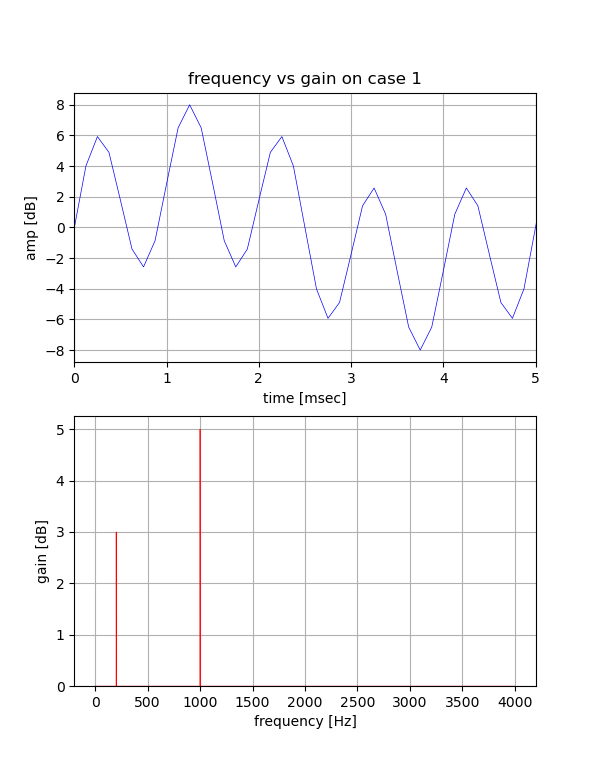
\includegraphics[width=0.4\linewidth]{../picture/case1.png}
  \caption{case1におけるDFT結果}
  \label{case1}
\end{figure}
図\ref{case1}からは,200Hzと1000Hzにピークを持つ振幅スペクトルが得られていることが確認できる.


\subsection{case2 100Hz,500Hz,2000Hzの正弦波の合成波}
case2で用いたデータを入力として,Pythonスクリプトを実行した応答を図\ref{case2}に示す.
処理は2.80秒で正常に終了した.
\begin{figure}[H]
  \centering
  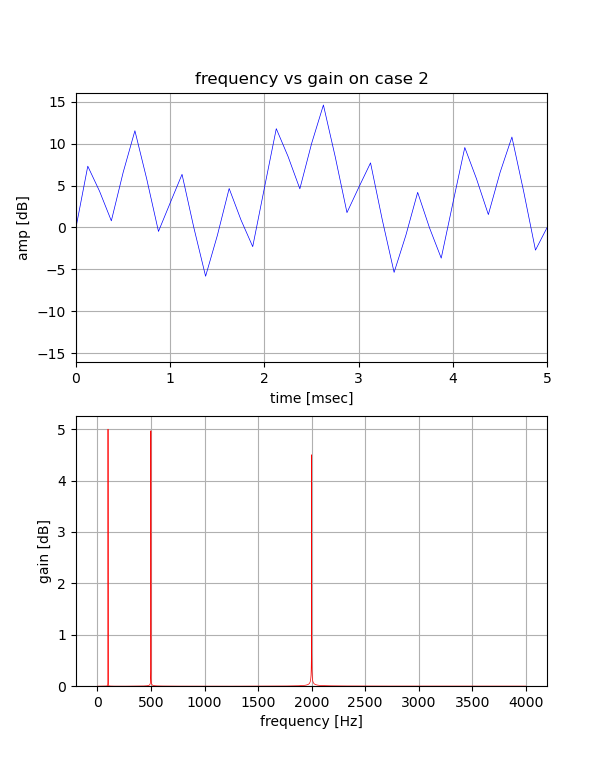
\includegraphics[width=0.4\linewidth]{../picture/case2.png}
  \caption{case2におけるDFT結果}
  \label{case2}
\end{figure}
図\ref{case2}からは,100Hz,500Hz,2000Hzにピークを持つ振幅スペクトルが得られていることが確認できる.

\subsection{結言}
case1,case2ともに入力に対し意図した変換を実施でき,作成したRust関数および可視化用Pythonスクリプトを用いて,正弦波の合成波の振幅スペクトルを正しく計算することができたといえる.

\begin{thebibliography}{99}
  \bibitem{toyama} 外山 茂浩、実験テキスト「フーリエ解析」、(2022年)
  \bibitem{nikkei} 日経BP、パワーコンディショナー(PCS)とは、\\https://project.nikkeibp.co.jp/ms/article/WORD/20130925/305286、(2013年10月)
  \bibitem{nikkei2} エネチェンジ、EV(電気自動車)の気になる充電!時間や場所、料金は?、\\https://enechange.jp/articles/ev-charging、(2021年12月19日)
\end{thebibliography}

\end{document}